%%%%%%%%%%%%%%%%%%%%%%%%%%%%%%%%%%%%%%%%%%%%%%%%%%%%%%%%%%%%%%%%%%%%%%%%
\chapter{Sistemi ideali di Fermi--Dirac}
\label{cap:fermi}
%%%%%%%%%%%%%%%%%%%%%%%%%%%%%%%%%%%%%%%%%%%%%%%%%%%%%%%%%%%%%%%%%%%%%%%%

Nel seguito per brevità mi riferirò a un sistema di Fermi--Dirac semplicemente
come a un sistema di Fermi.

%%%%%%%%%%%%%%%%%%%%%%%%%%%%%%%%%%%%%%%%%%%%%%%%%%%%%%%%%%%%%%%%%%%%%%%%
\section{Equazioni fondamentali per un gas ideale di Fermi}
%%%%%%%%%%%%%%%%%%%%%%%%%%%%%%%%%%%%%%%%%%%%%%%%%%%%%%%%%%%%%%%%%%%%%%%%

Cominciamo con lo scrivere le relazioni per la pressione $P$ e il numero medio
di particelle $N$ che abbiamo ricavato in precedenza:
\bea
\label{eq:fermifund}
\dfrac{PV}{kT} &\equiv& \ln\calQ = \sum_\eps\ln\left(1 + \zembe\right)
\nonumber\\
N &\equiv&\sum_\eps \langle n_\eps\rangle = \sum_\eps \dfrac{1}{\zmebe+1}
\eea
Contrariamente al caso di Bose, nel caso di Fermi $z$ può assumere qualsiasi
valore: $0 \le z < \infty$. Il principio di esclusione di Pauli fa sì che in
nessun livello di energia possano accumularsi più di $g$ particelle, in cui $g$
è il fattore di degenerazione dovuto allo spin (per particelle di spin $1/2$,
come gli elettroni, $g = 2$). Quindi non ci sarà nessun fenomeno simile alla
condensazione di Bose--Einstein, e non dobbiamo preoccuparci di trattare in
maniera particolare il livello $\eps =0$, come abbiamo fatto nel caso di Bose.
Il comportamento quantistico di un gas di Fermi è completamente diverso da
quello di un gas di Bose, ma non per questo meno interessante.

Senza ripetere tutti i passaggi che portano dalle somme (\ref{eq:fermifund})
agli integrali, passaggi che sono in tutto e per tutto simili a quelli che
abbiamo visto nel capitolo precedente, a parte un segno meno di differenza,
scriviamo direttamente i risultati fondamentali:
\bea
\label{eq:fermifundint}
\dfrac{P}{kT} &=& \dfrac{g}{\lambda^3}\,\fFD{5/2}(z) \nonumber\\
\dfrac{N}{V}  &=& \dfrac{g}{\lambda^3}\,\fFD{3/2}(z)
\eea
in cui abbiamo messo ``a mano'' il fattore di degenerazione $g$ e abbiamo
introdotto le funzioni di Fermi--Dirac
\be
\label{eq:deffFD}
\fFD{\nu}(z) = \dfrac{1}{\Gamma(\nu)}\int_0^\infty\de x
\dfrac{x^{\nu-1}}{\zmex+1}
\ee
Allo stesso modo delle funzioni $\gBE{\nu}(z)$, anche le funzioni di
Fermi--Dirac ammettono uno sviluppo in serie, ma stavolta a segni alterni:
\be
\label{eq:expFD}
\fFD{\nu}(z) = z - \dfrac{z^2}{2^\nu} + \dfrac{z^3}{3^\nu} - \cdots
= \sum_{s=1}^\infty (-1)^{s-1} \dfrac{z^s}{s^\nu}
\ee
%%%%%%%%%%%%%%%%%%%%%%%%%%%%%%%%%%%%%%%%%%%%%%%%%%%%%%%%%%%%%%%%%%%%%%%%
\begin{Exercise}[title={Espansione delle funzioni di Fermi},
label={ex:fermiexp}]
Dimostrare la (\ref{eq:expFD}).

[{\em Suggerimento}\ Vedi l'esercizio equivalente per le funzioni di
Bose]$\quad\bullet$
\end{Exercise}
%%%%%%%%%%%%%%%%%%%%%%%%%%%%%%%%%%%%%%%%%%%%%%%%%%%%%%%%%%%%%%%%%%%%%%%%
\noindent
Eliminando la $z$, le (\ref{eq:fermifundint}) permettono in linea di principio
di scrivere l'equazione di stato di un gas ideale di Fermi.

%%%%%%%%%%%%%%%%%%%%%%%%%%%%%%%%%%%%%%%%%%%%%%%%%%%%%%%%%%%%%%%%%%%%%%%%
\section{Espansione del viriale}
%%%%%%%%%%%%%%%%%%%%%%%%%%%%%%%%%%%%%%%%%%%%%%%%%%%%%%%%%%%%%%%%%%%%%%%%

Analogamente al caso di Bose, possiamo scrivere, per l'energia interna,
\bea
\label{eq:defUFD}
U &=& -\bfrac{\partial\ln\calQ}{\partial\beta}_{z,V} =  
kT^2\left[\dparu{T}\bfrac{PV}{kT}\right]_{z,V} \nonumber\\
&=& kT^2 gV \fFD{5/2}(z)\dfrac{\de\lambda^{-3}}{\de T} = 
\dfrac{3}{2}kT\dfrac{gV}{\lambda^3}\fFD{5/2}(z) =
\dfrac{3}{2}NkT\dfrac{\fFD{5/2}(z)}{\fFD{3/2}(z)}
\eea
e otteniamo la solita relazione tra pressione e energia interna:
\be
\label{eq:relUPFD}
P = \dfrac{2U}{3V}
\ee

\textbf{TODO}

%%%%%%%%%%%%%%%%%%%%%%%%%%%%%%%%%%%%%%%%%%%%%%%%%%%%%%%%%%%%%%%%%%%%%%%%
\section{Il limite di degenerazione}
%%%%%%%%%%%%%%%%%%%%%%%%%%%%%%%%%%%%%%%%%%%%%%%%%%%%%%%%%%%%%%%%%%%%%%%%

Nel limite $T\to 0$, il valor medio dei numeri d'occupazione diventa
\be
\aspne = \dfrac{1}{e^{(\mu-\eps)/kT} + 1} = \left\{ \begin{array}{ll}
 1 & \eps <\mu_0\\
 0 & \eps >\mu_0
  \end{array} \right.
\ee
in cui $\mu_0$ è il valore del potenziale chimico a $T=0$. La funzione $\aspne$
diventa una funzione a gradino. Tutti i livelli di energia con $\eps < \mu_0$
sono riempiti, e tutti i livelli di energia con $\eps > \mu_0$ sono vuoti. Al
valore limite $\mu_0$, che gioca un ruolo importantissimo in molti sistemi
fisici, viene dato il nome di {\em energia di Fermi} del sistema, indicata dal
simbolo $\eps_F$. Il corrispondente valore del momento, il {\em momento di
Fermi}, si indica con $p_F$.

Per calcolare $\eps_F$, scriviamo prima di tutto l'equazione generale per il
numero medio di particelle $N$:
\be
N = \int_0^\infty \de\eps \, a(\eps) \aspne
\ee
in cui $a(\eps)$ è la solita densità degli stati (non--relativistica) del
sistema, moltiplicata per il fattore di degenerazione di spin, $g$:
\be
a(\eps) = \dfrac{gV}{h^3}2\pi(2m)^{3/2}\eps^{1/2}
\ee
Nel limite $T\to0$ $\aspne$ può essere sostituita con la funzione a gradino:
quindi
\be
\dfrac{N}{V}= \dfrac{1}{V}\int_0^{\eps_F} \de\eps\,a(\eps) = \dfrac{4\pi
g(2m)^{3/2}}{3h^3}\eps_F^{3/2}
\ee
da cui otteniamo facilmente
\be
\label{eq:computEF}
\eps_F = \dfrac{h^2}{2m}\bfrac{3n}{4\pi g}^{2/3}
\ee
e, per il momento di Fermi,
\be
\label{eq:computePF}
p_F = h\bfrac{3n}{4\pi g}^{1/3}
\ee
Per l'energia di punto zero, ossia l'energia del sistema quando $T\to 0$,
troviamo un valore diverso da zero; cosa che è nettamente in contrasto col
comportamento di un gas ideale classico, in cui l'energia interna va a zero
linearmente con la temperatura. Per essere specifici possiamo scrivere
\be
E_0 = \int_0^{\eps_F}\de\eps\,\eps\,a(\eps)
= \dfrac{2\pi g(2m)^{3/2} V}{h^3}\int_0^{\eps_F}\de\eps\,\eps^{3/2}
= \dfrac{4\pi gV(2m)^{3/2}}{5h^3}\eps_F^{5/2}
\ee
Se ora dividiamo per $N$ otteniamo
\be
\dfrac{E_0}{N} = \dfrac{3}{5}\eps_F
\ee
Utilizzando la relazione tra pressione e energia interna, che vale a qualsiasi
temperatura, otteniamo
\be
P_0 = \dfrac{2E_0}{3V} = \dfrac{2}{5}n\eps_F
\ee
Considerando che $\eps_F\propto n^{2/3}$ otteniamo che $P_0\propto n^{5/3}$.
Sembra proprio che anche allo zero assoluto il gas di Fermi continui a
esercitare una certa attività. Tutto questo è dovuto al principio di esclusione
di Pauli, quindi a un fenomeno puramente quantistico. Questo peculiare
comportamento del gas di Fermi nel limite degenere $(T\to 0)$ spiega, come
vedremo, parecchi fenomeni fisici che resterebbero altrimenti misteriosi.

Una volta definita l'energia di Fermi di un sistema, possiamo anche definire la
sua {\em temperatura} di Fermi:
\be
T_F = \eps_F/k
\ee
Quando la temperatura di un sistema costituito da fermioni è molto inferiore
alla sua temperatura di Fermi, il caso degenere costituisce una buona
approssimazione del sistema stesso.

%%%%%%%%%%%%%%%%%%%%%%%%%%%%%%%%%%%%%%%%%%%%%%%%%%%%%%%%%%%%%%%%%%%%%%%%
\section{Espansione a bassa temperatura}
%%%%%%%%%%%%%%%%%%%%%%%%%%%%%%%%%%%%%%%%%%%%%%%%%%%%%%%%%%%%%%%%%%%%%%%%

Come nel caso dei sistemi di Bose, per valori intermedi di $z$ l'unica
soluzioneconsiste nel risolvere le equazioni numericamente. Quando
$n\lambda^3\to 0$
possiamo ricorrere all'espansione del viriale, e quando $T=0$ possiamo fare i
conti esattamente, trovando una prima approssimazione nel caso di piccole
temperature. Il calcolo però del calore specifico, per esempio, richiede una
temperatura anche solo leggermente diversa da zero, per poter fare la derivata
rispetto alla temperatura stessa. Dobbiamo ricorrere a un'espansione a bassa
temperatura per poter calcolare le prime correzioni al caso degenere.

In figura (\ref{fig:nefd}) è mostrato l'andamento qualitativo di $\aspne$ per
tre valori della temperatura, $T_2 < T < T_1$ (le unità di misura sono
altamentearbitrarie). Vediamo che a temperatura $T_2$ la funzione $\aspne$ si
avvicina a
una funzione a gradino.
%%%%%%%%%%%%%%%%%%%%%%%%%%%%%%%%%%%%%%%%%%%%%%%%%%%%%%%%%%%%%%%%%%%%%%
\begin{figure}[!ht]
	\centering
	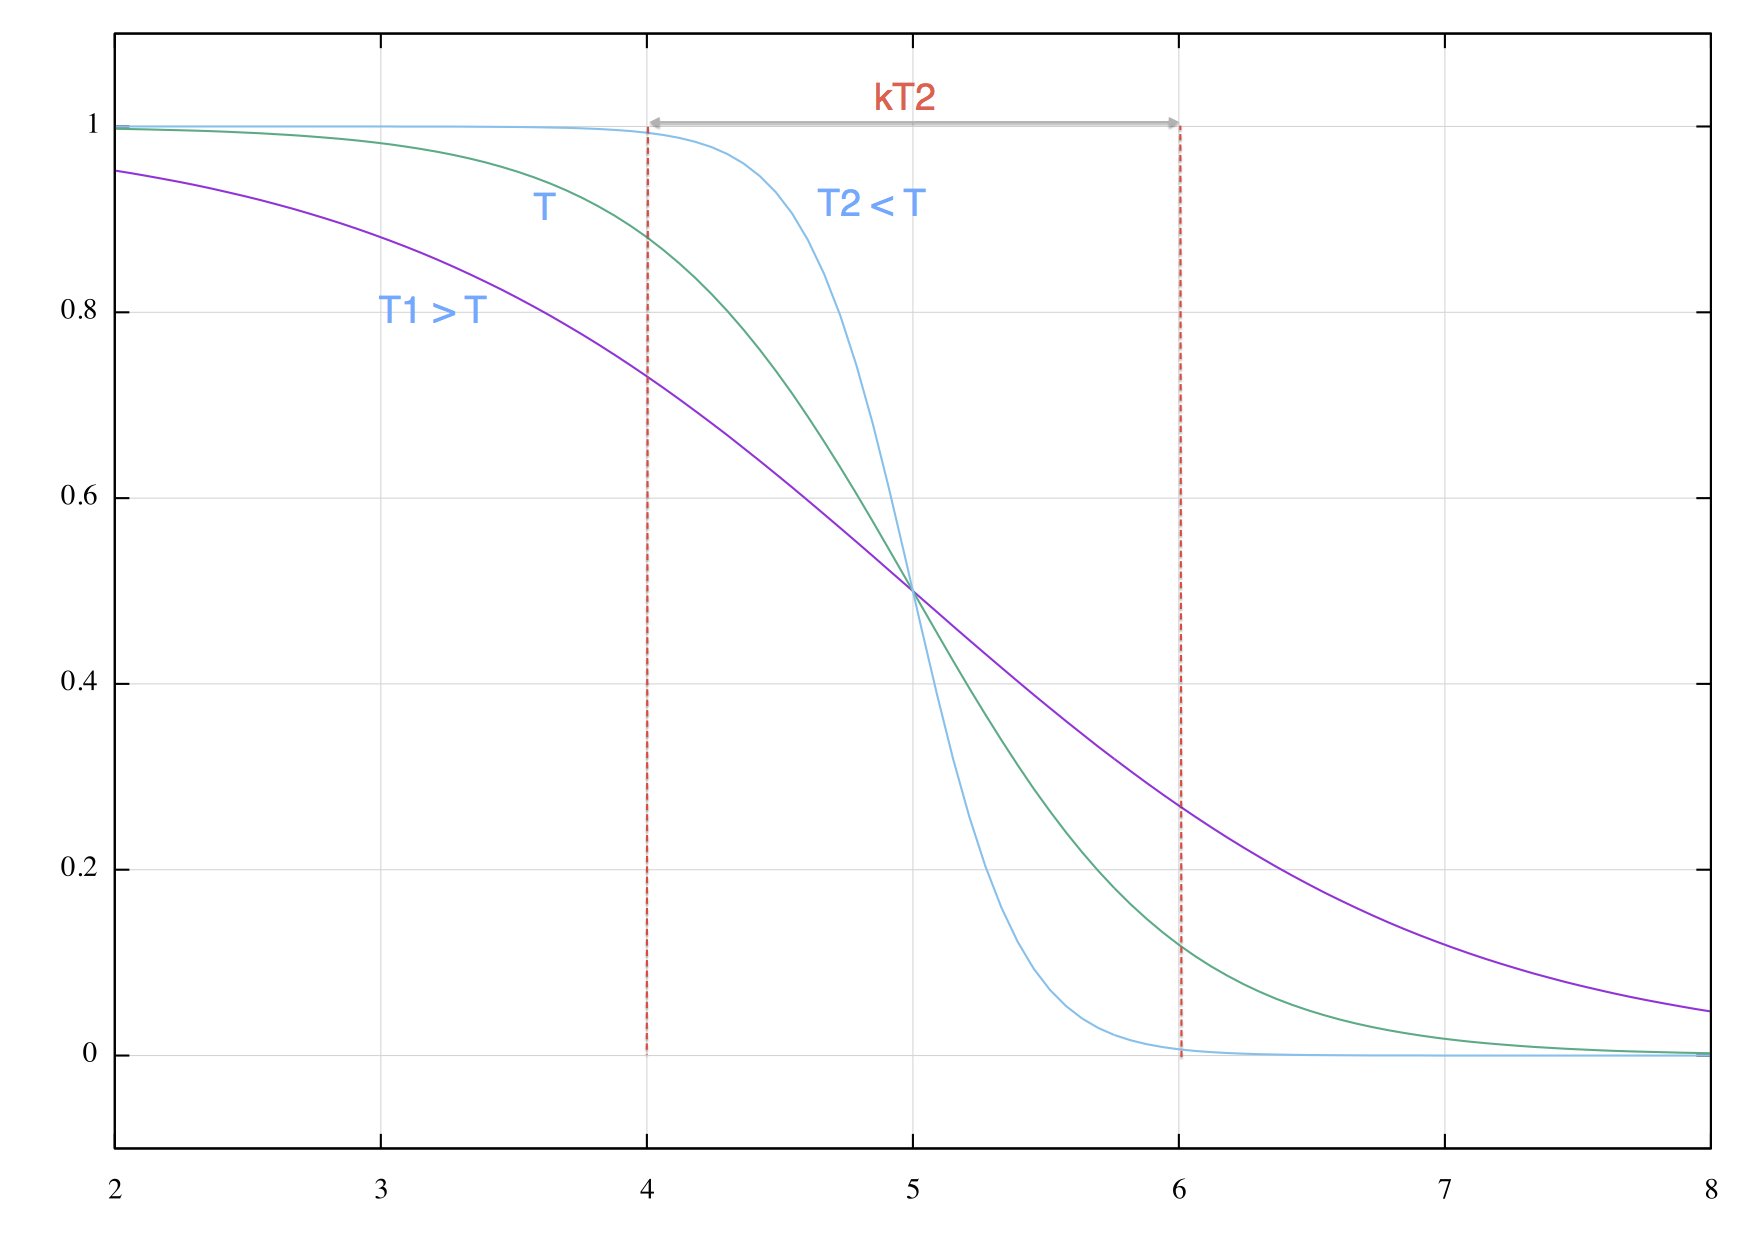
\includegraphics[width=1.0\textwidth]{nefd.png}
	\caption{Andamento qualitativo di $\aspne$ per la statistica di Fermi.}
	\label{fig:nefd}
\end{figure}
%%%%%%%%%%%%%%%%%%%%%%%%%%%%%%%%%%%%%%%%%%%%%%%%%%%%%%%%%%%%%%%%%%%%%%
\noindent
Per un valore $T$ della temperatura, la funzione $\aspne$ differisce in maniera
significativa da $0$ e da $1$ solo in un intervallo che ha un ordine di
grandezza $O(kT)$. Un argomento euristico ma profondo per capire questo
comportamento è il seguente: a temperatura $T$ l'energia termica che possiamo
fornire a una particella è proprio $O(kT)$. Se la particella si trova in un
livello di energia $\eps$ molto più basso di $\eps_F$ allora non può saltare al
livello $\eps+kT$, semplicemente perché lo trova già occupato. Solo le
particelle che si trovano a una distanza $O(kT)$ dal livello di Fermi possono
saltare per andare a occupare stati non ancora occupati, sopra il livello di
Fermi, ma a loro volta non possono andare più lontano di $O(kT)$, perché solo
quella è l'energia a disposizione. Questo argomento può essere reso più
rigoroso, come mostra il seguente esercizio.
%%%%%%%%%%%%%%%%%%%%%%%%%%%%%%%%%%%%%%%%%%%%%%%%%%%%%%%%%%%%%%%%%%%%%%
\begin{Exercise}
Si consideri un sistema costituito da fermioni a una temperatura $T \ll T_F$;
$T_F$ è la temperatura di Fermi del sistema. Si calcoli in quale intervallo la
funzione $\aspne$ è significativamente diversa da $0$ e da $1$.

\noindent
[{\em Suggerimento } Approssimare $\aspne$ con una spezzata e calcolare la
derivata prima di $\aspne$ nel punto di flesso, che corrisponde a
$\eps_F$]$\quad\bullet$
\end{Exercise}
%%%%%%%%%%%%%%%%%%%%%%%%%%%%%%%%%%%%%%%%%%%%%%%%%%%%%%%%%%%%%%%%%%%%%%

Fortunatamente le funzioni di Fermi ammettono un'espansione a bassa
temperatura.I dettagli possono essere trovati nell'appendice \textbf{TODO}. In
realtà a
temperatura $T=0$ il valore di $z$ è $\infty$. A piccole temperature le
funzioni$\fFD{\nu}(z)$ possono essere espresse come un'espansione asintotica in
potenze
di $(\,\ln z\,)^{-1}$. Per i valori di $\nu$ cui siamo interessati otteniamo
\bea
\fFD{5/2}(z) &=& \dfrac{8}{15\pi^{1/2}}(\,\ln z\,)^{5/2}\left[   
1 + \dfrac{5\pi^2}{8}(\,\ln z\,)^{-2} + \cdots
\right] \nonumber\\
\fFD{3/2}(z) &=& \dfrac{4}{3\pi^{1/2}}(\,\ln z\,)^{3/2}\left[   
1 + \dfrac{\pi^2}{8}(\,\ln z\,)^{-2} + \cdots
\right] \nonumber\\
\fFD{1/2}(z) &=& \dfrac{2}{\pi^{1/2}}(\,\ln z\,)^{1/2}\left[   
1 - \dfrac{\pi^2}{24}(\,\ln z\,)^{-2} + \cdots
\right]
\eea
Armati di queste espansioni otteniamo facilmente
\be
\dfrac{N}{V} = \dfrac{4\pi g}{3}\bfrac{2m}{h^2}^{3/2}(\,kT\ln z\,)^{3/2}\left[ 
1 + \dfrac{\pi^2}{8}(\,\ln z\,)^{-2} + \cdots\right]
\ee
che nell'approssimazione zero ci dà
\be
kT\ln z \equiv \mu \simeq \bfrac{3n}{4\pi g}\dfrac{h^2}{2m}
\ee
risultato identico, ovviamente, a quello del caso degenere: $\mu_0 = \eps_F$.
All'ordine successivo otteniamo
\be
\label{eq:muexpf}
kT\ln z \equiv \mu \simeq \eps_F \left[ 
1 - \dfrac{\pi^2}{12}\bfrac{kT}{\eps_F}^{2}\right]
\ee
Per la densità di energia interna abbiamo
\be
\dfrac{U}{N} = \dfrac{3}{5}(\,kT\ln z\,)\left[ 
1 + \dfrac{\pi^2}{2}(\,\ln z\,)^{-2} + \cdots\right]
\ee
che con l'aiuto della (\ref{eq:muexpf}) diventa
\be
\label{eq:ufd}
\dfrac{U}{N} = \dfrac{3}{5}\eps_F\left[ 
1 + \dfrac{5\pi^2}{12}\bfrac{kT}{\eps_F}^{2} + \cdots\right]
\ee
e da questa ricaviamo subito la pressione:
\be
P = \dfrac{2U}{3V} = \dfrac{2}{5}n\eps_F\left[ 
1 + \dfrac{5\pi^2}{12}\bfrac{kT}{\eps_F}^{2} + \cdots\right]
\ee
Infine, derivando la (\ref{eq:ufd}) rispetto a $T$ tenendo $z$, $N$ e $V$
costanti, otteniamo
\be
\dfrac{C_V}{Nk} = \dfrac{\pi^2}{2}\dfrac{kT}{\eps_F} + \cdots =
\dfrac{\pi^2}{2}\dfrac{T}{T_F} + \cdots
\ee
Vediamo quindi che per gas ideali di Fermi il calore specifico va a zero
linearmente con $T/T_F$. Questo risultato ci sarà molto utile in seguito, per
spiegare il calore specifico dei metalli.

%%%%%%%%%%%%%%%%%%%%%%%%%%%%%%%%%%%%%%%%%%%%%%%%%%%%%%%%%%%%%%%%%%%%%%
\section{Fenomeni magnetici in un gas di Fermi ideale}
%%%%%%%%%%%%%%%%%%%%%%%%%%%%%%%%%%%%%%%%%%%%%%%%%%%%%%%%%%%%%%%%%%%%%%

È interessante studiare il comportamento dei fermioni in presenza di un campo
magnetico. Ci aspettiamo che la statistica di Fermi--Dirac modifichi in maniera
sostanziale i risultati che abbiamo ottenuto studiando, per esempio, il
paramagnetismo con la statistica di Maxwell--Boltzmann. Le nostre aspettative
non andranno deluse. Abbiamo visto che classicamente troviamo la legge di
Curie,ossia il fatto che la suscettività magnetica è proporzionale a $T^{-1}$
nel
limite di alte temperature; a basse temperature otteniamo invece una
saturazionemagnetica completa. Sperimentalmente questo non è quel che si
osserva. Gli
elettroni in banda di conduzione nei metalli alcalini dovrebbero formare nel
metallo, in prima approssimazione, un gas ideale; quel che si osserva, invece
della situazione classica, è un paramagnetismo estremamente debole che non
mostra saturazione a basse temperature. Questo fenomeno è stato compreso da
Pauli nel 1927 sulla base della statistica di Fermi--Dirac.

Un altro fenomeno che è completamente incomprensibile dal punto di vista
classico è il diamagnetismo, ossia il fatto che un gas di elettroni acquisisce
una magnetizzazione che è di verso contrario a quello del campo magnetico.
Questo fenomeno fu spiegato da Landau nel 1930, e la spiegazione ha a che fare
con la quantizzazione delle orbite degli elettroni in un campo magnetico
esternoperpendicolare al piano dell'orbita stessa. Questo porta a una
suscettività
negativa. Per comprendere il comportamento magnetico di alcuni materiali è
dunque necessario prendere in considerazione entrambi gli effetti.

%%%%%%%%%%%%%%%%%%%%%%%%%%%%%%%%%%%%%%%%%%%%%%%%%%%%%%%%%%%%%%%%%%%%%%
\subsection{Paramagnetismo di Pauli}
%%%%%%%%%%%%%%%%%%%%%%%%%%%%%%%%%%%%%%%%%%%%%%%%%%%%%%%%%%%%%%%%%%%%%%

Sia $m$ la massa di una particella di spin $1/2$, $\musb$ il suo momento
magnetico intrinseco e $\mathbf{B}$ un campo magnetico esterno. L'energia di
singola particella, in questo caso, è data da
\be
\eps = \dfrac{p^2}{2m} - \musb \cdot \mathbf{B}
\ee
Il vettore $\musb$ sarà o parallelo o antiparallelo al vettore $\mathbf{B}$.
Nelgas troveremo dunque due gruppi di particelle:
\begin{enumerate}
\item[i)] il gruppo di particelle con $\musb$ parallelo a $\mathbf{B}$ ed
energia $\eps = \dfrac{p^2}{2m} - \mu^*B$;
\item[ii)] il gruppo di particelle con $\musb$ antiparallelo a $\mathbf{B}$ ed
energia $\eps = \dfrac{p^2}{2m} + \mu^*B$.
\end{enumerate}
A $T=0$ tutti i livelli di energia fino a $\eps_F$ saranno pieni, mentre tutti
ilivelli con energia superiore saranno vuoti. Di conseguenza l'energia {\em
cinetica} del primo gruppo di particelle andrà da $0$ a $(\eps_F + \mu^*B)$,
mentre quella del secondo andrà da $0$ a $(\eps_F - \mu^*B)$.

Chiamiamo $N^+$ il numero di particelle nel primo gruppo e $N^-$ il numero di
particelle nel secondo gruppo; usando le formule standard del caso
completamentedegenere otteniamo
\bea
N^+ &=& \dfrac{4\pi V (2m)^{3/2}}{3h}\left[ \eps_F + \mu^*B \right]^{3/2}
\nonumber \\
N^- &=& \dfrac{4\pi V (2m)^{3/2}}{3h}\left[ \eps_F - \mu^*B \right]^{3/2}
\eea
Il momento magnetico netto posseduto dal sistema sarà
\bea
M &=& \mu^* (N^+ - N^-) \nonumber \\
  &=& \dfrac{4\pi \mu^* V (2m\eps_F)^{3/2}}{3h}\left\{
\left[ 1 + \dfrac{\mu^*B}{\eps_F} \right]^{3/2} - 
\left[ 1 - \dfrac{\mu^*B}{\eps_F} \right]^{3/2}
\right\}
\eea
Per campo debole possiamo espandere $(1 \pm x)^\alpha \simeq 1 \pm \alpha x$
ottenendo
\be
\chi_0 = \lim_{B \to 0} \dfrac{M}{VB} = \dfrac{4\pi \mu^{*2} V
(2m)^{3/2}\eps_F^{1/2}}{h^3}
\ee
Ricordando l'espressione (\ref{eq:computEF}) possiamo scrivere
\be
\chi_0 = \dfrac{3}{2} n \mu^{*2} / \eps_F
\ee
in cui $n = N/V$; dunque una suscettività costante e soppressa da $\eps_F$.

Per ottenere un'espressione (approssimata) di $\chi$ valida a tutte le
temperature dobbiamo seguire una via un po' tortuosa. Chiamiamo
$n^+_{\mathbf{p}}$ il numero di particelle con momento $\mathbf{p}$ e momento
magnetico parallelo al campo magnetico, e $n^-_{\mathbf{p}}$ il numero di
particelle con momento $\mathbf{p}$ e momento magnetico antiparallelo al campo
magnetico. In virtù della statistica di Fermi devono ovviamente valere i
vincoli\be
\label{eq:npnm}
n^+_{\mathbf{p}}\;,\, n^-_{\mathbf{p}} = 0 \; \mathrm{o} \; 1
\ee
e
\be
\label{eq:NpNm}
\sum_{\mathbf{p}} n^+_{\mathbf{p}} + \sum_{\mathbf{p}}n^-_{\mathbf{p}} = N^+ +
N^- = N
\ee

L'energia totale del sistema sarà evidentemente data da
\bea
E_n &=& \sum_{\mathbf{p}} \left[
\left( \dfrac{p^2}{2m} - \mu^* B \right) n^+_{\mathbf{p}} +
\left( \dfrac{p^2}{2m} + \mu^* B \right) n^-_{\mathbf{p}}
\right] \nonumber \\
&=& \sum_{\mathbf{p}} \left[
\left( n^+_{\mathbf{p}} + n^-_{\mathbf{p}} \right) \dfrac{p^2}{2m}
\right] - \mu^* B (N^+ - N^+)
\eea
e la funzione di partizione del sistema sarà
\be
Q(N) = \sideset{}{'}\sum_{\{n^+_{\mathbf{p}}\}\{n^-_{\mathbf{p}}\}} e^{-\beta
E_n}
\ee
in cui l'apice sulla somma ci ricorda che la somma stessa, su tutti i possibili
stati, è sottoposta ai vincoli (\ref{eq:npnm}) e (\ref{eq:NpNm}). Per calcolare
la funzione di partizione $Q_N$, prima di tutto fissiamo un valore arbitrario
per il numero $N^+$; ciò fissa automaticamente anche $N^-$. A questo punto
sommiamo su tutti i possibili valori di $n^+_{\mathbf{p}}$ e $n^+_{\mathbf{p}}$
che sono conformi, oltre al vincolo (\ref{eq:npnm}), anche al valore fissato di
$N^+$ e $N^-$. Infine sommiamo su tutti i possibili valori di $N^+$, cioè da
$0$a $N$. Abbiamo dunque
\bea
\label{eq:QNPauliParam}
Q(N) &=& \sum_{N^+=0}^N
e^{\beta\mu^* B(2N^+ - N)}  \times \nonumber \\
&\ & \left[
\sideset{}{''}\sum_{\{n^+_{\mathbf{p}}\}}
\exp\left(-\beta\sum_{\mathbf{p}}\dfrac{p^2}{2m}n^+_{\mathbf{p}}\right)
 \sideset{}{'''}\sum_{\{n^-_{\mathbf{p}}\}}
\exp\left(-\beta\sum_{\mathbf{p}}\dfrac{p^2}{2m}n^-_{\mathbf{p}}\right)
\right]
\eea
in cui la somma $\sum''$ è soggetta al vincolo 
$\sum_{\mathbf{p}}n^+_{\mathbf{p}} = N^+$
mentre la somma $\sum'''$ al vincolo
$\sum_{\mathbf{p}}n^-_{\mathbf{p}} = N-N^+$.

Consideriamo ora un gas ideale di $N_0$ particelle di massa $m$ che obbediscono
alla statistica di Fermi--Dirac; queste particelle sono però ``senza spin''.
Anche se questa è chiaramente una {\em finzione}, nessuno potrà impedirci di
fare i conti. Per la funzione di partizione $Q_0(N_0)$ di questo sistema
fittizio otteniamo
\be
Q_0(N_0) = \sideset{}{'}\sum_{n_{\mathbf{p}}}
\exp \left(
-\beta \sum_{\mathbf{p}} \dfrac{p^2}{2m}n_{\mathbf{p}}
\right) \equiv e^{-\beta A_0(N_0)}
\ee
in cui per definizione $A_0(N_0)$ è l'energia libera del sistema stesso. Risulta evidente che l'eq. (\ref{eq:QNPauliParam}) può essere riscritta come
\be
Q(N) = e^{-\beta\mu^* BN}\sum_{N^+=0}^N
\left[
e^{2\beta\mu^* BN^+} Q_0(N^+) Q_0(N-N^+)
\right]
\ee
dalla quale ricaviamo subito
\bea
&&\dfrac{1}{N}\ln Q(N) = -\beta \mu^* B \nonumber \\
&+& \dfrac{1}{N}\ln \sum_{N^+=0}^N \exp
\left\{
2\beta \mu^* B N^+ - \beta A_0(N^+) - \beta A_0(N-N^+)
\right\}
\eea
Come abbiamo più volte fatto in passato, approssimiamo il logaritmo della somma con il logaritmo del termine più grande della somma stessa; l'errore {\em relativo} commesso, nel limite termodinamico, risulta trascurabile. Il termine più grande della somma si otterrà per un valore di $N^+$ pari a $\bar{N}^+$, e per trovarlo massimizziamo rispetto a $N^+$; otteniamo
\be
2 \mu^* B - 
\dparc{A_0(N^+}{N^+}{N^+=\bar{N}^+} -
\dparc{A_0(N-N^+}{N^+}{N^+=\bar{N}^+}
= 0
\ee
cioè
\be
\label{eq:mu0PauliParam}
\mu_0(\bar{N}^+) - \mu_0(N-\bar{N}^+) = 2 \mu^* B
\ee
in cui evidentemente $\mu_0(N_0)$ è il potenziale chimico del sistema fittizio di $N_0$ fermioni senza spin. Per la magnetizzazione totale, per definizione, avremo
\be
M = \mu^*
\left(
\bar{N}^+ - \bar{N}^-
\right) = \mu^*
\left(
2\bar{N}^+ - N
\right)
= \mu^* N r
\ee
in cui abbiamo introdotto il parametro $r \equiv 2\bar{N}^+/N - 1$, con $0 \le r \le 1$. L'equazione (\ref{eq:mu0PauliParam}) diventa
\be
\label{eq:mu0rPP}
\mu_0
\left(
\dfrac{1+r}{2}N
\right)
-
\mu_0
\left(
\dfrac{1-r}{2}N
\right)
=
2 \mu^* B
\ee
Se il campo magnetico è nullo, allora anche $r$ sarà nullo, perché in assenza di campo magnetico dovremo avere, in media, $\bar{N}^+ = \bar{N}^-$. Quindi per campo magnetico piccolo possiamo espandere intorno a $r=0$:
\bea
\mu_0
\left(
\dfrac{1+r}{2}N
\right)
\simeq \mu_0(N/2) + \dfrac{r}{2}\dparc{\mu_0(xN)}{x}{x=1/2} + \cdot \nonumber \\
\mu_0
\left(
\dfrac{1-r}{2}N
\right)
\simeq \mu_0(N/2) - \dfrac{r}{2}\dparc{\mu_0(xN)}{x}{x=1/2} + \cdot
\eea
e sottraendo membro a membro otteniamo, ricordando la (\ref{eq:mu0rPP}),
\be
r \simeq \dfrac{2\mu^* B}{\dparc{\mu_0(xN)}{x}{x=1/2}}
\ee
Dunque per campo debole la suscettività per unità di volume è
\be
\chi = \dfrac{M}{VB} = \dfrac{\mu^* N r}{V B} = \dfrac{2n\mu^*}{\dparc{\mu_0(xN)}{x}{x=1/2}}
\ee
Questo è il risultato che cercavamo, valido per ogni temperatura.

Per $T\to 0$, il potenziale chimico del sistema fittizio è l'energia di Fermi di detto sistema:
\be
\mu_0(xN) =
\left(
\dfrac{3xN}{4\pi V}
\right)^{2/3}\dfrac{h^2}{2m}
\ee
da cui ricaviamo facilmente
\be
\dparc{\mu_0(xN)}{x}{x=1/2} = \dfrac{2^{4/3}}{3}
\left(
\dfrac{3N}{4\pi V}
\right)^{2/3}\dfrac{h^2}{2m}
\ee
D'altra parte sappiamo ben scrivere l'energia di Fermi per il sistema fisico sotto esame:
\be
\eps_F =
\left(
\dfrac{3N}{8\pi V}
\right)^{2/3}\dfrac{h^2}{2m}
\ee
e con l'aiuto delle ultime due equazioni ricaviamo
\be
\chi_0 = \dfrac{3}{2} n \mu^{*2} / \eps_F
\ee
in completo accordo con nostro precedente risultato a $T = 0$. 

%%%%%%%%%%%%%%%%%%%%%%%%%%%%%%%%%%%%%%%%%%%%%%%%%%%%%%%%%%%%%%%%%%%%%%
\subsection{Diamagnetismo di Landau}
%%%%%%%%%%%%%%%%%%%%%%%%%%%%%%%%%%%%%%%%%%%%%%%%%%%%%%%%%%%%%%%%%%%%%%

Per quest'anno il diamagnetismo di Landau e l'effetto termoionico non sono in programma. Questo non vi impedisce di portarli come argomento a piacere.

